\documentclass[a4paper,12pt]{article}
%\usepackage[latin1]{inputenc}
\usepackage[T1]{fontenc}
\usepackage[utf8]{inputenc}
\usepackage{calc}
\usepackage{setspace}
%\usepackage{fixltx2e}
\usepackage{graphicx}
\usepackage{multicol}
\usepackage{textcomp} %to avoid a warning generated by gensymb
\usepackage{gensymb}
\usepackage[normalem]{ulem}
%% Please revise the following command, if your babel
%% package does not support fr-CA
%\usepackage[frenchb]{babel}
\usepackage[round,authoryear,sort&compress]{natbib}
\usepackage[UKenglish]{babel}
\usepackage{caption}
%\usepackage{subcaption} %cannot be used together with subfig!
\usepackage{color}
\usepackage{hyperref}

\usepackage{eurosym}
\usepackage{lastpage}
\usepackage{vhistory}
%\usepackage[style=authoryear,natbib=true,maxcitenames=1]{biblatex}
\usepackage{amsmath, amsthm, amssymb, amsfonts}
\usepackage{xurl} %added by FK

\usepackage{coverpage_reuniwatt}
\usepackage{multirow}

\usepackage{indentfirst}

\newcommand\MyBox[2]{
  \fbox{\lower0.75cm
    \vbox to 1.7cm{\vfil
      \hbox to 1.7cm{\hfil\parbox{1.4cm}{#1\\#2}\hfil}
      \vfil}%
  }%
}
  
\usepackage[
  top=2cm,
  bottom=3cm,
  left=3cm,
  right=3cm,
  headheight=33.33pt, % as per the warning by fancyhdr
  headsep=2cm,
  includehead,includefoot,
  heightrounded, % to avoid spurious underfull messages
]{geometry} 
  
  
%Reuniwatt header and footer
\usepackage{fancyhdr}
\pagestyle{fancy}
\fancyhf{}
\renewcommand\headrule{}
\renewcommand{\footrulewidth}{1pt}
\renewcommand{\footrule}{\hbox to\headwidth{\color{red}\leaders\hrule height \headrulewidth\hfill}}

\fancyfoot[CE,CO]{\footnotesize Reuniwatt SAS, 14 rue de la Guadeloupe, 97490 Sainte-Clotilde\\
Tel : 06.92.64.43.13 / Fax : 02.62.92.10.20 / courriel : info@reuniwatt.com\\
Soci\'{e}t\'{e} par Actions Simplifi\'{e}e au capital de 191.700\euro\ RCS Saint-Denis 518 919 345}

\rhead{Page \thepage/\pageref{LastPage}}
\lhead{
\includegraphics[scale=0.2]{reuniwatt.jpg}}



%\renewcommand \vhChangeColWidth{1.2\hsize}
%\renewcommand \vhAuthorColWidth{2\hsize}

%titre
\title{Internship report}

\hyphenation{Re-uni-watt Bar-quiss-eau Ra-dio-sound-ing} %custom hyphenation list
\setlength\parindent{0pt} %FK edit: no indent at beginning of paragraph
 
\begin{document}
\hbadness=10000  %FK edit: less warnings for underfull/overfull hboxes

\maketitle
\addtocounter{page}{1}

\setcounter{table}{0}
\newpage
\tableofcontents
\newpage

\section*{Abstract}
\addcontentsline{toc}{section}{Abstract}

For day-ahead forecasting, the combination of Numerical Weather Prediction (NWP) models and post-processing algorithms is the most popular method.

However, it is hard to extract from all the literature on the subject the best algorithm to use because of the lack of consistency in the different approaches.
Indeed different works use different datasets, metrics and even cross-validation methods. 

During my internship, my mission was to investigate the best algorithms according to the literature so as to improve the day-ahead irradiance forecasts. 
The comparison is initially conducted on 4 sites over the years 2021 and 2022, and aims at post-processing GFS forecasts data so as to lower both the mean average error (MAE) and the root mean square error (RMSE).
I eventually studied the hybridation of different forecast NWP models (AROME, GFS, ARPEGE, ECMWF), on 25 more validation sites, in order to benchmark it against the current algorithm used by Reuniwatt.

My final results demonstrated the benefits of post-processing both a single NWP model and several NWP models altogether.
While a linear model perform good enough for a RMSE optimisation, a support vector regression (SVR) model proved its ability to lower the MAE.
The ultimate model showcased improved metrics with respect to the current algorithm used by Reuniwatt.

\newpage

\section{Introduction}
\subsection{Background and motivation of the intership project}
This report is the result of my 6-month internship in Reuniwatt, a leader in cloud observation and forecasting.
My internship extended from March 1st to August 31st, taking place during the second semester of my academic gap.

The main subject of the intership was the post-processing of the day ahead NWP irradiance forecasts.
Despite their proven utility for day-ahead irradiance forecasting, NWP models predictions can still be improved thanks to post-processing.

As I will show in \ref{subsec:models}, many models have been investigated in the literature, and it is thus important to draw a clean benchmark
of all the available state-of-the-art models.

Statistical models will be investigated, whose applications do not restrict to day-ahead irradiance forecasts. Indeed any timestamped weather-related variable could benefit
of the post-processing I am going to discuss in this paper.
\subsection{Objectives of the internship}
Hereafter the main objectives of the internship:
\begin{itemize}
    \item Benchmark promising models on the post-processing of a single NWP model.
    \item Sensitivity study of the models.
    \item Comparison of the results with the current model used by Reuniwatt for day-ahead forecasting (LT CONT).
\end{itemize}
\newpage

\section{Methodology}
\label{sec:methodo}
\subsection{Data source}
\cite{verbois_statistical_2022} demonstrated that using a large set of predictors can significantly improve the performances of post-processing models, while \cite{suksamosorn_post-processing_2021}
selected WRF forecasts of irradiance, temperature, relative humidity and the solar zenith angleas relevant inputs of the models.

Our initial data source for the forecasts was GFS, and we opted for the following set of predictors (\ref{tab:set_pred}), both simple and easily available for any location.

The forecasted data is for each day the one relative to the origin 00:00 UTC of the day before. The irradiance explored during my internship is the global horizontal irradiance (GHI), which is
the total solar radiation incident on a horizontal surface.

\begin{table}[h]
    \centering
    \begin{tabularx}{\textwidth} { 
  | >{\centering\arraybackslash}X 
  | >{\centering\arraybackslash}X 
  | >{\centering\arraybackslash}X 
  | >{\centering\arraybackslash}X
  | >{\centering\arraybackslash}X 
  |}
 \hline
 $ghi_{GFS}$ & $T_{GFS}^{2m}$ & $\theta$ & $\phi$ & $ghi_{cs}$ \\
 \hline
 \scriptsize Irradiance forecasted  & \scriptsize Temperature forecasted 2 meters above the ground & \scriptsize Zenith angle & \scriptsize Azimuth angle & \scriptsize Clear-sky irradiance \\
\hline
\end{tabularx}
    \caption{Set of predictors.}
    \label{tab:set_pred}
\end{table}

\cite{verbois_statistical_2022} advises researchers to analyze their models performances over several years but I was at this point limited by the Reuniwatt API, thus
I initially opted for learning during 2020 and testing during 2021.

The four initial study sites are the following (\ref{fig:initial_sites}):
\begin{figure}[htb!]
    \centering
    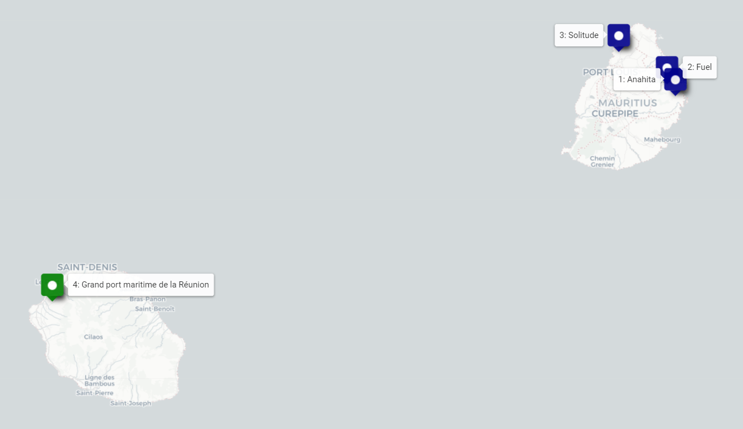
\includegraphics[width=0.7\textwidth]{figures/initial_study_sites.png}
    \caption{Four initial study sites}
    \label{fig:initial_sites}
\end{figure}
\subsection{Metrics}
Even if papers like \cite{mayer_calibration_2023} state that the correlation coefficient is the recommended metrics to use when no clear directive is given, the metrics 
that I am going to investigate are the one already prefered by Reuniwatt, the mean absolute error (MAE) and the root mean square error (RMSE). 

I also wanted to investigate the MBE optimization, but the results were not convincing and MBE is more seen in our study as a metrics to be verified after post-processing.
We indeed aim at the lowest absolute MBE.

\begin{itemize}
    \item The mean absolute error \begin{align*}
        MAE = \frac{1}{N} \sum_{i=1}^{N} | I_{forecast, i} - I_{measure, i} |
    \end{align*}

    \item The mean bias error \begin{align*}
        MBE = \frac{1}{N} \sum_{i=1}^{N} ( I_{forecast, i} - I_{measure, i} )
    \end{align*}

    \item The root mean square error \begin{align*}
        RMSE = \sqrt{\frac{1}{N} \sum_{i=1}^{N} ( I_{forecast, i} - I_{measure, i} ) ^{2}}
    \end{align*}

    \item The skill score $s$  of a certain accuracy measure $A$, with R denoting the reference irradiance
    \begin{align*}
        s = 1 - \frac{A(X,Y)}{A(R,Y)}
    \end{align*}
\end{itemize}

\subsection{Models investigated}\label{subsec:models}
Our bibliography study leads us toward the most relevant models to be tested.

Concerning the reference model, \cite{lorenz_benchmarking_nodate} and others suggested the use of the persistence model, consisting in taking as prediction the latest measure available,
but this model turned out to have too poor results to be a good reference model. I opted for using the raw forecasted value as the reference model.

\cite{suksamosorn_post-processing_2021} proposed a really interesting linear model based on a Kalman filter scheme. Hence the Kalman filter was first used as a promising linear model to be 
assessed against heavier non-linear machine learning models.

On the hand of machine learning models, \cite{verbois_statistical_2022} distinguished the models effective to reduce the RMSE, including multi-layer perceptron (MLP) and gradient boosting machine (GBM),
and the models promising for reducing the MAE, notably the standard vector regression (SVR).
\cite{suksamosorn_post-processing_2021} also pointed out the effectiveness of the random forest (RF) model for a RMSE-optimization.

It's why I am going to compare the following models, against the reference raw forecasted irradiance.
\begin{itemize}
    \item Kalman filter model (KF).

The Kalman filter is a recursive estimator. This means that only the estimated state from the previous time step and the current measurement are needed to compute the estimate for the current state.

The correction procedure involves two groups of equations: time update equations
and measurements update equations, time update equations are responsible for making
a first guess of the next solar irradiance prediction error, based on the last state of the
measured error and error covariance estimates, obtaining an a priori prediction for the next
time step; the measurement update equations will then incorporate new measurements
into the first guess, obtaining improved a posteriori predictions.

My understanding of the general Kalman filter was greatly thanks to \cite{kfbasis}, and I practised the filter thanks to \cite{kfpractise}.

In the context of irradiance forecasting, I followed the path from \cite{suksamosorn_post-processing_2021}.
    \item Gradient boosting machine model (GBM).
GBM creates an ensemble of weak learners, meaning that it combines several smaller, simpler models in order to obtain a more accurate prediction than what an individual model would produce. Gradient boosting works by iteratively training the weak learners on gradient-based functions and incorporating them into the model as “boosted” participants. 

For more information, see notably \cite{GBMbasis} for the theory and \cite{GBMpractise} for the python practise.
    \item Support vector regression model (SVR).

    The support vector regression method is often used in cases where there are multiple input variables, each of which may have an effect on the output variable. The goal is to find the best linear combination of these input variables to predict the output variable.

To estimate the coefficients of the linear function, standard vector regression uses a method called least squares regression. This involves finding the values of the coefficients that minimize the sum of the squared differences between the predicted and actual values.
    Here is an interesting article on the subject: \cite{SVR}.
    \item Random forest model (RF).

    The Random Forest algorithm is an ensemble method used for machine learning. It creates multiple decision trees, each trained on a different subset of data and considering random features for splitting. The final prediction is made by combining the predictions of these trees through voting (for classification) or averaging (for regression), resulting in improved accuracy and reduced overfitting.

Again, here is a link for a hands-on practise of the RF algorithm: \cite{RF}.
    \item Multiple-layer perceptron model (MLP).

The Multilayer Perceptron (MLP) is a type of artificial neural network used in machine learning. It consists of multiple layers of interconnected nodes (neurons) where each node computes a weighted sum of its inputs, passes it through an activation function, and then forwards the result to the next layer. MLPs are commonly used for various tasks such as classification, regression, and pattern recognition, and they can learn complex relationships in data. They can be trained using backpropagation, adjusting the weights between nodes to minimize the difference between predicted and actual outputs.

\end{itemize}
All this models will be compared during the internhip, and all the data wrangling architecture around it can be found either in the README or more specifically in the source code of my repo \cite{myrepo}.

After having post-processed a single NWP forecast model individually, the next step will be to assess the performances of our hybrid model in comparison to the one currently used by Reuniwatt (LT CONT).
\subsection{Model performances evaluation strategy}
The benchmarking consists in evaluating the performances on each metrics of each one of the model optimized with the corresponding metrics.

A grid search which details can be explored in \cite{myrepo} is used for the learning year in order to find the best hyperparameters for any of the model.

We assess the performances of the trained models on their performances on the test year.

The big picture will be given by a global significance matrix that will compare all the models performances regarding the particular metrics across the 4 sites.
This matrix will allow us to discern the most pertinent models for each of our study metrics.
Then, to verify that the models indeed perform well in the detail and across the different times of the day, we are going to plot scatter plots and data distributions of the MBE for each site.

This dual approach will ensure us that global results indeed translate into improved performances for each hour of the day, and especially in term of bias (MBE).
\newpage

\section{Results and discussion}
% Define a custom command to create sections with shared structure

As explained in \autoref{sec:methodo}, the first objective is to effectively post-process a single NWP forecast model, by benchmarking the models altogether. 

The following step will be to look at the results in the details to prove the true effectiveness of the post-processing.

We will each time first study the MAE optimisation and then the RMSE optimisation. Be aware that the models hyperparameters may vary between the two optimisations because the 
target metrics to minimize is not the same during the computations.
\subsection{Post-processing of a single forecasting NWP model}
\subsubsection{Study of the models altogether} 
\paragraph{MAE}\indent
\begin{figure}[htb!]
    \centering
    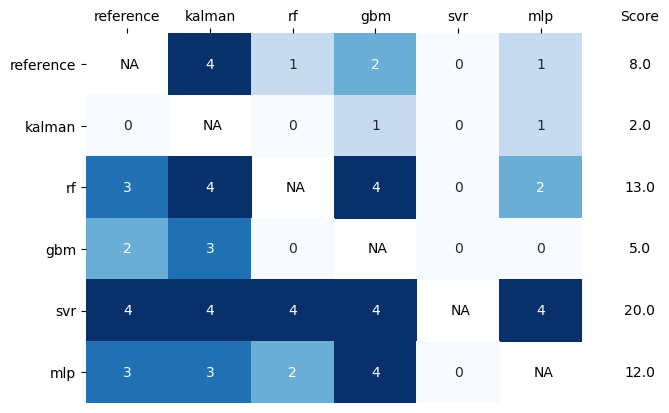
\includegraphics[width=\columnwidth]{figures/first_study/significance_matrix_mae.png}
\caption{Significance matrix for MAE. The value $V_{(i,j)}$ of the $(i,j)$ cell indicates how often the model of line i performs better than the one of column j, across the 
4 sites. For example, the MAE of the MLP model post-processed data is 3 times lower than the MAE of the reference model, and for 1 site (4 - 3 = 1), it is higher.}
\label{fig:sig_mae}
\end{figure}

\begin{figure}[htb!]
    \centering
    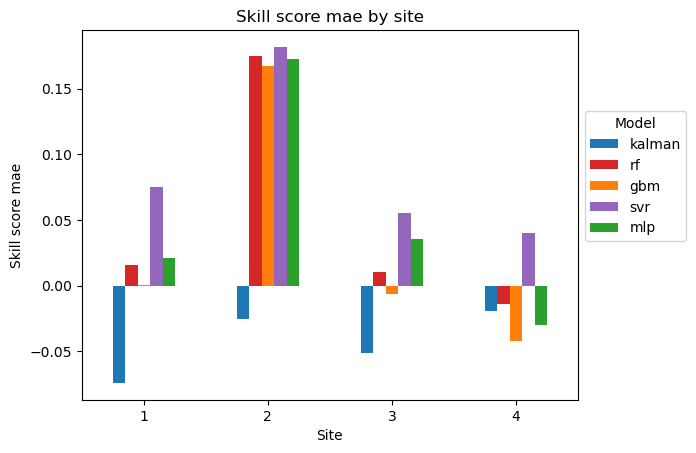
\includegraphics[width=\columnwidth]{figures/first_study/ss_mae.png}
    \caption{MAE skill score plot across the 4 sites.}
\label{fig:ss_mae}
\end{figure}
\autoref{fig:sig_mae} clearly shows that the SVR model is the best one for MAE. It performs better than any of the other model on any of the 4 study cases.

\autoref{fig:ss_mae} demonstrates that the sites 1, 3 and 4 heavily benefit from this model with respect to the other ones. 
On site 4, the only positive post-processing is given by the SVR model.

The Kalman filter showcases really poor performances across the 4 sites.

\newpage
\paragraph{RMSE}\indent

\begin{figure}[htb!]
    \centering
    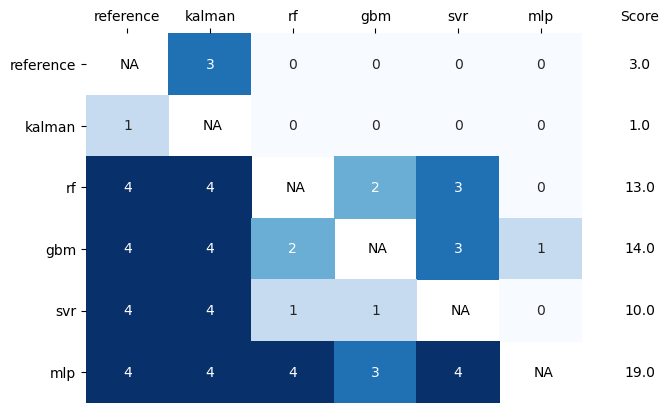
\includegraphics[width=\columnwidth]{figures/first_study/significance_matrix_rmse.png}
\caption{Significance matrix for RMSE. The value $V_{(i,j)}$ of the $(i,j)$ cell indicates how often the model of line i performs better than the one of column j, across the 
4 sites. For example, the RMSE of the MLP model post-processed data is 3 times lower than the RMSE of the reference model, and for 1 site (4 - 3 = 1), it is higher.}
\label{fig:sig_rmse}
\end{figure}

\begin{figure}[htb!]
    \centering
    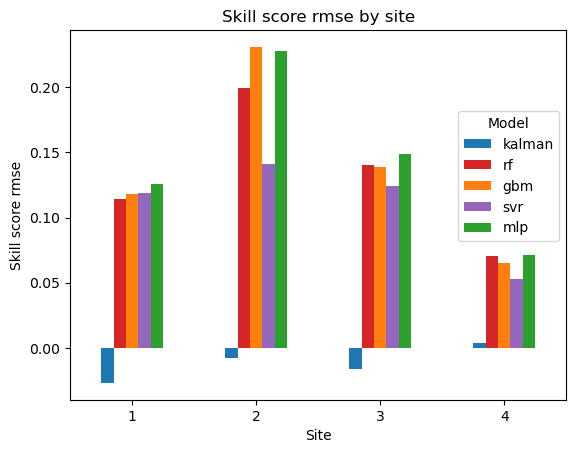
\includegraphics[width=0.75\columnwidth]{figures/first_study/ss_rmse.png}
    \caption{RMSE skill score plot across the 4 sites.}
    \label{fig:ss_rmse}
\end{figure}

The results of the RMSE are not the same, and it is the MLP model that performs the best, achieving the highest score in the matrix of \autoref{fig:sig_rmse}.

This is confirmed by \autoref{fig:ss_rmse} where the MLP model bar is the highest for 3 sites out of 4.

\subsubsection{Detailled study of the most performing model}
With the aim of clarity, only the plots of the single site 2 will be shown here.
The overall similarity of the results across the 4 sites also motivate this choice.

The ones of the other sites can be found in the appendix to fortify the belief in the analysis drawn for a single site.

\paragraph{MAE}\indent
\begin{figure}[htb!]
    \centering
    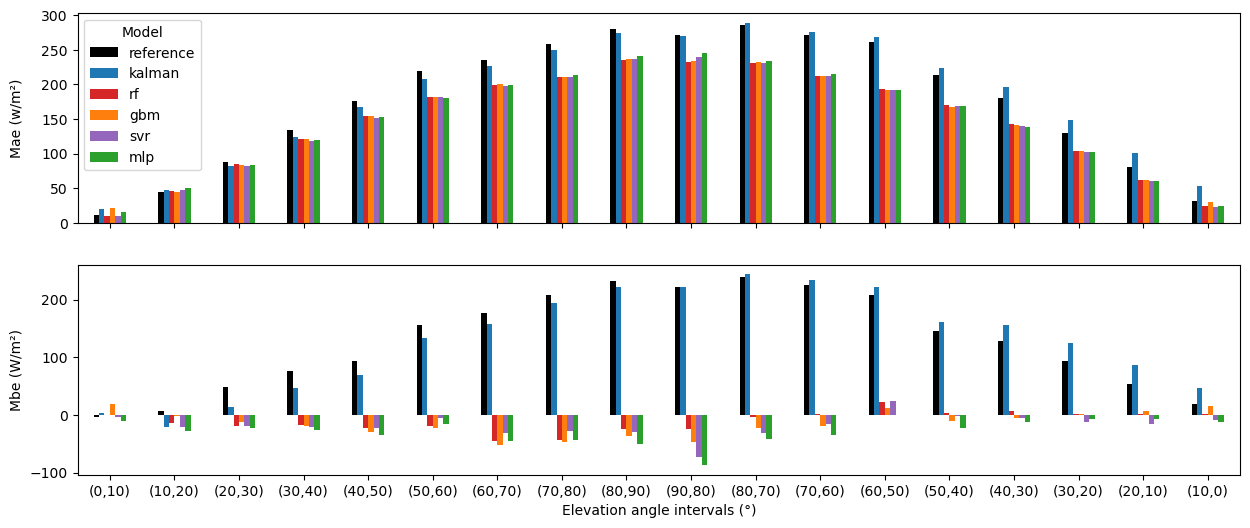
\includegraphics[width=\columnwidth]{figures/first_study/mae_mbe_site2.png}
\caption{MAE and MBE levels across all elevation angle intervals of a day, for site 2.}
\label{fig:mae_mbe_site2}
\end{figure}

    \autoref{fig_mae_mbe_site2} supports our previous conclusions, but most importantly shows the decrease of the MBE across all the elevation angle intervals of a day.
Indeed, it is a know fact that NWP models present a positive bias that is higher around noon, and the MBE of all the machine learning models tends to be much closer to 0.

On site 2, the bias is negative but this bias can be either positive or negative depending on the study site, as confirmed with the other graphs in \autoref{appendix:single}.
Only site 4 shows a different behavior for the bias across the day, but this does not change the MAE results. 
\begin{figure}[htb!]
    \centering
    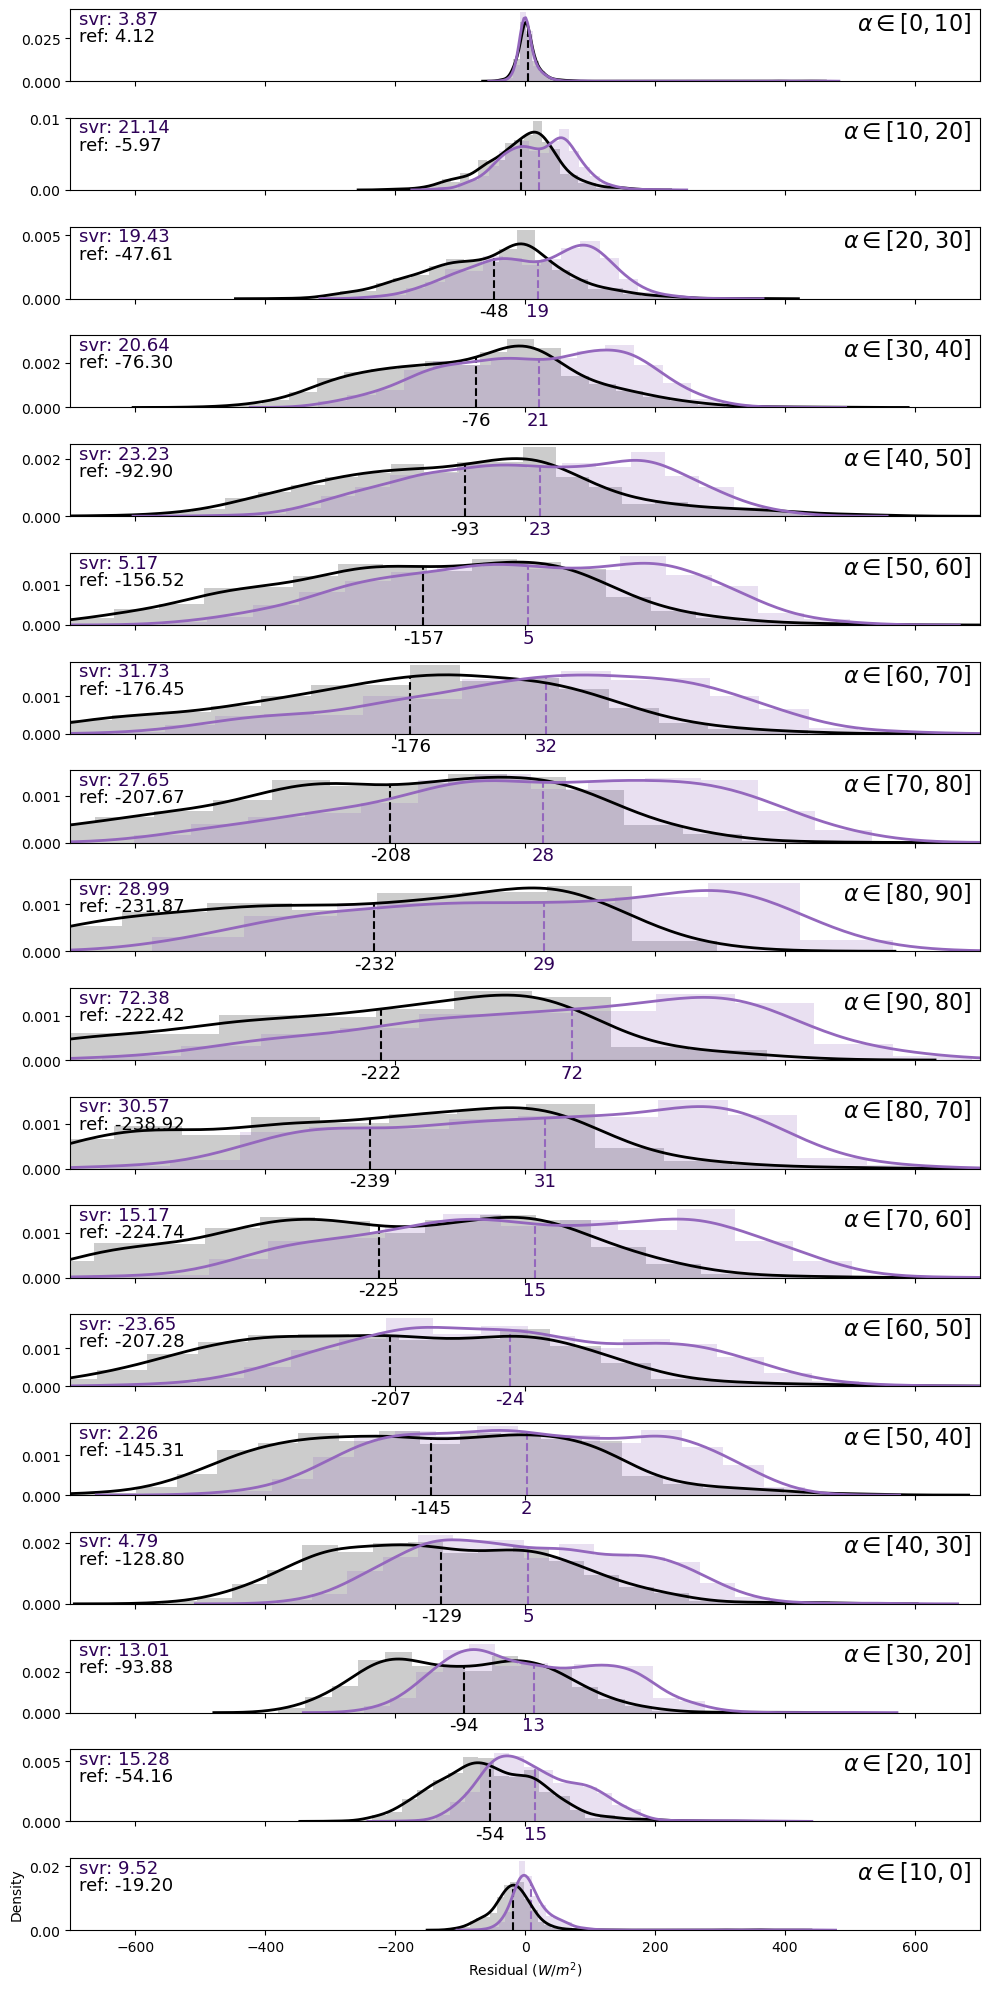
\includegraphics[width=\columnwidth]{figures/first_study/residual_errors_svr_site2_mae.png}
\caption{Residual error levels across all elevation angle intervals of a day, for a SVR model, for site 2.}
\end{figure}

The probability density functions across the day support these conclusions, where we can clearly see that the curve is shifted towards 0, as are the scatter plots in \autoref{appendix:single}.
The whole dataset cloud is shifted towards the line y=x, which is the line where the corrected forecast exactly match the measured irradiance.\\

These plots about the MAE minimisation thanks to the SVR model show that this model is not only able to reduce the MAE across the day, but also to reduce the MBE across the day.

The global lowering of the global metrics is indeed reflected in the lowering of the metrics at each elevation angle interval of particular day. The bias is also improved in 3 sites out of 4.
\paragraph{RMSE}\indent

Similar conclusions can be drawn about the RMSE minimisation, with the MLP model.

The only difference is that the improvement of the MBE now stands for all the study cases.

\begin{figure}[htb!]
    \centering
    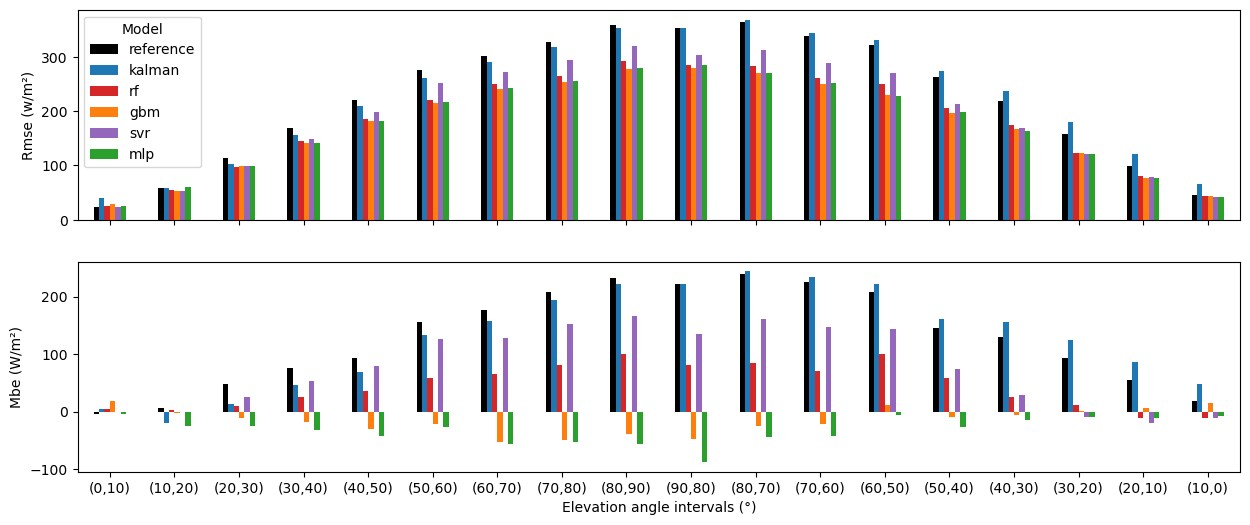
\includegraphics[width=\columnwidth]{figures/first_study/rmse_mbe_site2.png}
\caption{RMSE and MBE levels across all elevation angle intervals of a day, for site 2.}
\end{figure}

\begin{figure}[htb!]
    \centering
    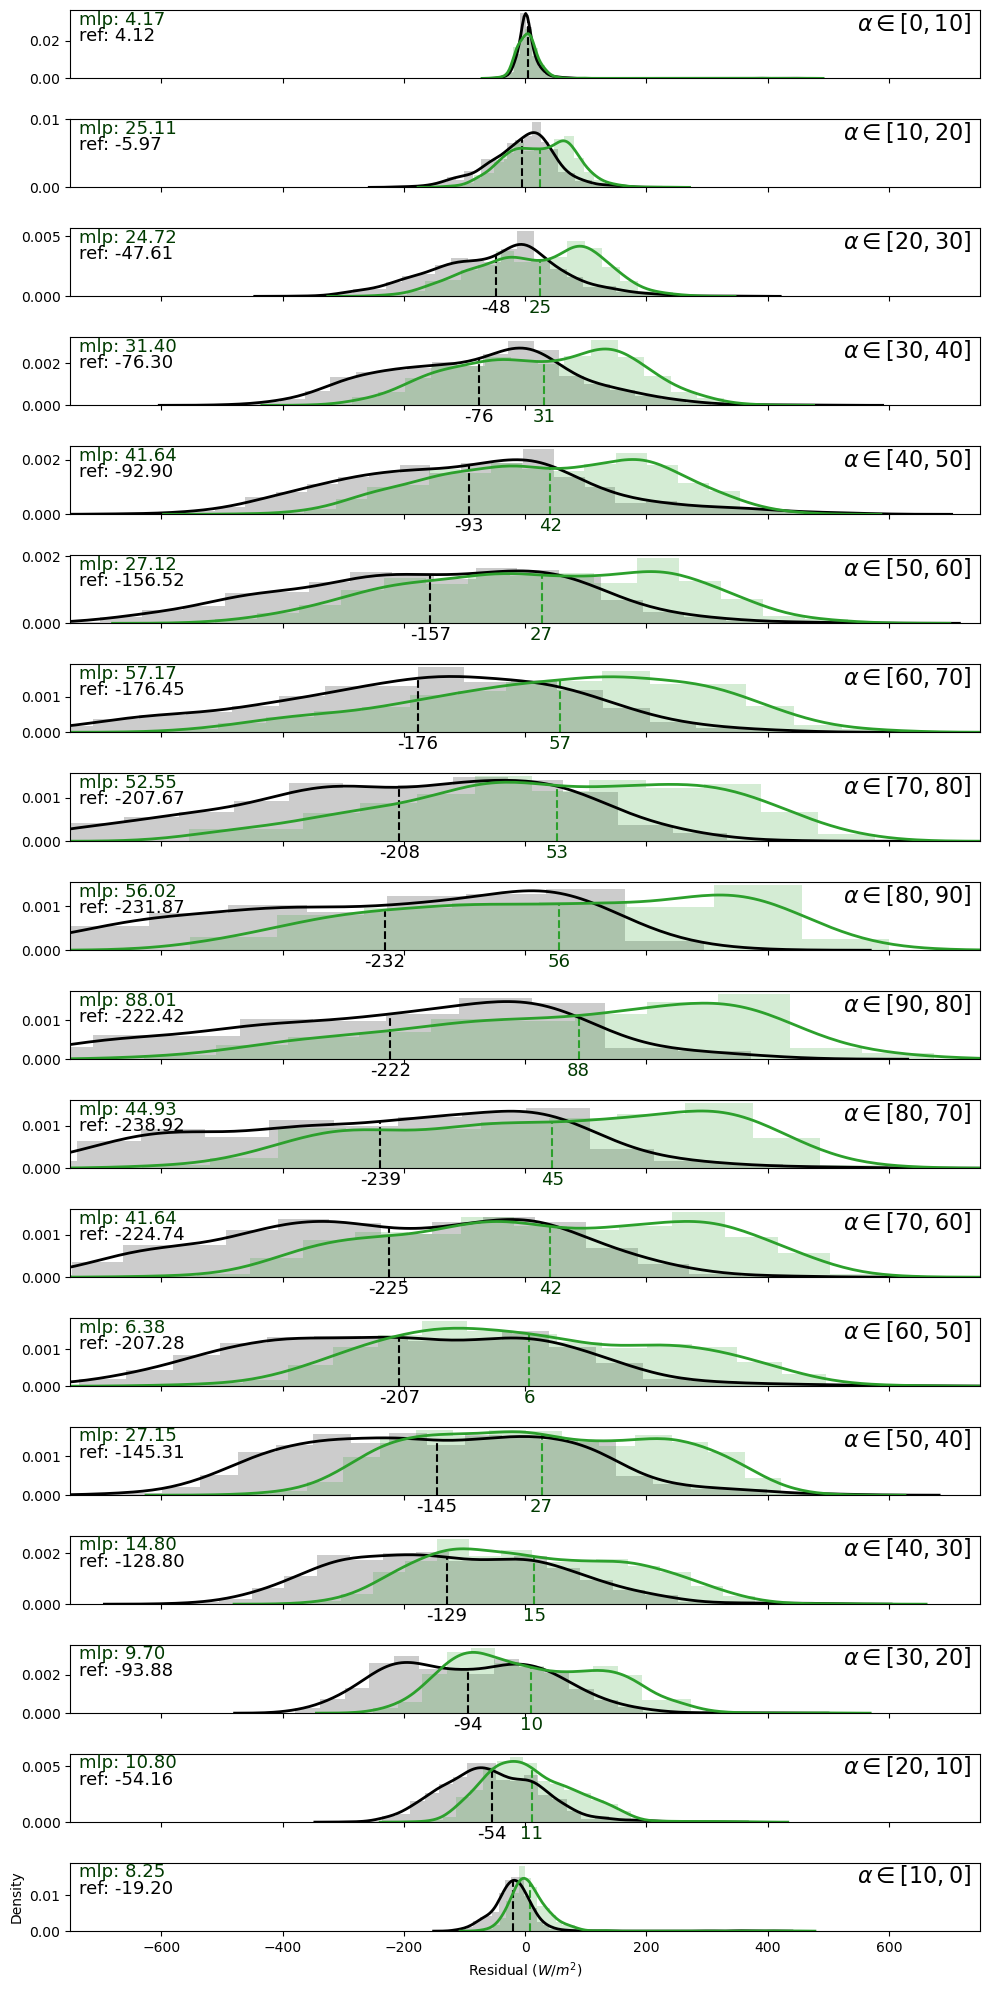
\includegraphics[width=\columnwidth]{figures/first_study/residual_errors_mlp_site2_rmse.png}
\caption{Residual error levels across all elevation angle intervals of a day, for a MLP model, for site 2.}
\end{figure}

All in all, the improvement of the metrics of interest (MAE and RMSE) is reflected in an improvement of the bias. 

This behavior stands for each period of a day, which was not perfectly obvious after I performed the global post-processing.\\

Once the relevant models have been found, one has to perform a sensitivity study of these ones in order to better grasp how they work.

\subsubsection{Sensitivity study}
It is also necessary to perform a sensitivity study of the parameters that are not tuned in our process. It is why the influence of the choices of predictors, of learning periods, of learning window type (fixed or sliding) and of forecasting model are successively performed. 

With the aim of clarity, the results will be here presented with the MAE optimisation, but the results of the RMSE optimisation lead the same conclusions, and can also
be found in \autoref{appendix:single}.

\paragraph{Influence of the choice of the predictors}
The first sensitivity study is performed with the set of predictors that was presented in \autoref{tab:set_pred}.
\begin{table}[htb!]
\begin{center}
\begin{tabular}{|l|llll|}
\toprule
{} &  0 &  1 &  2 &  3 \\
\midrule
$ghi_{GFS}$            &  X &  X &  X &  X \\
$temperature^{2m}_{GFS}$ &  X &  X &    &    \\
$\theta$             &  X &  X &  X &    \\
$\phi$            &  X &  X &  X &    \\
$ghi_{cs}$             &  X &    &  X &    \\
\bottomrule
\end{tabular}
\end{center}
\label{tab:pred_configs}
\caption{Description of the configurations of the sets of predictors.}
\end{table}

\begin{figure}[htb!]
    \centering
    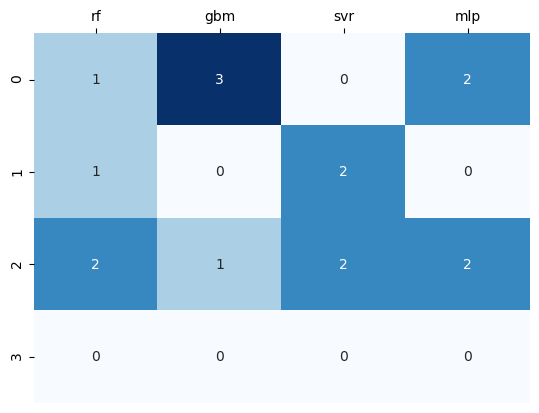
\includegraphics[width=\columnwidth]{figures/first_study/comp_predictors_mae.png}
\caption{Pairwise systematicity matrix for MAE. The value $V_{i,j}$ of the cell $(i,j)$ indicates how often the configuration of line i is the best one, across the 4 sites, for the model of column j. For example, the configuration 0 is the best one with a GBM post-processing for 3 sites, and the configuration 2 is the best one for 1 site.}
\label{fig:matrix_pred}
\end{figure}

\begin{figure}[htb!]
    \centering
    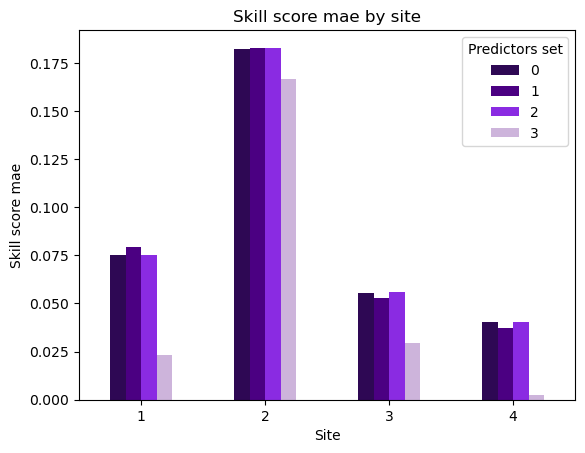
\includegraphics[width=\columnwidth]{figures/first_study/comp_predictors_mae_svr.png}
\caption{Comparison of the MAE skill scores of the different configurations.}
    \label{fig:ss_pred}
\end{figure}

Interestingly, the configuration with all the predictors is not the configuration that seem to give the best results if we consider \autoref{fig:matrix_pred}.

If we consider now \ref{fig:ss_pred}, the performances of the configurations 0, 1 and 2 are nearly identical. They both provide great improvements to the post-processing using only the forecasted irradiance.

In the following, I chose to always rely on the full configuration of the set of predictors. This is because I was working with only 5 predicting values and a feature selection is generally not advised when working with so few predictors.
This is a strong choice that could be questioned if the situation made to work with much more predictors (more than 10), where a feature selection would be necessary, both for metrics and computational performances reasons.
\paragraph{Influence of the learning period}

\begin{figure}[htb!]
    \centering
    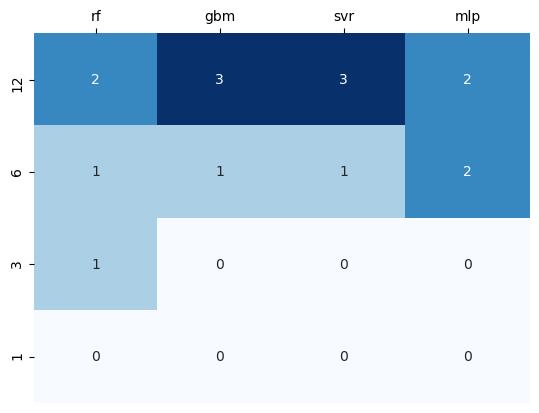
\includegraphics[width=\columnwidth]{figures/first_study/comp_learning_period_mae.png}
\caption{Pairwise systematicity matrix for MAE. The value $V_{i,j}$ of the cell $(i,j)$ indicates how often the learning period duration (in months) of line i performs the best, across the 4 sites, for the model of column j. For example, having a 12-months-long learning period is the best thing in 3 sites out of 4 with a SVR model, the last site performs better with a 6-month-long learning period.}
\label{fig:matrix_period}
\end{figure}

\begin{figure}[htb!]
    \centering
    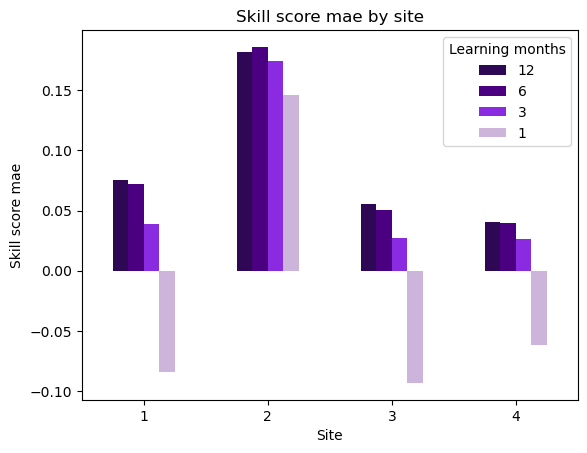
\includegraphics[width=\columnwidth]{figures/first_study/comp_learning_period_mae_svr.png}
    \label{fig:ss_period}
\caption{Comparison of the MAE skill scores of the different learning period durations (in months).}
\end{figure}

Both \autoref{fig:matrix_period} and \autoref{fig:ss_period} go to show that a larger learning period is beneficial for the model, up to one year when 
the benefits from increasing the learning period do not prove to be significant.

It is interesting to notice that a one-month learning period provides a negative post-processing.
\paragraph{Influence of the window of learning}
 
Another question from Reuniwatt was the pertinence of a sliding learning window.

I thus performed two types of learning:
\begin{itemize}
    \item A fixed-window learning where the testing period was the full year of 2021 and and the learning period was the full year of 2020.
    \item A sliding-window learning where each month of the test 2021 year used a model trained during the moving year that preceded this month. For instance, March 2021 used a model trained from February 2020 to February 2021.
\end{itemize}

\begin{figure}[htb!]
    \centering
    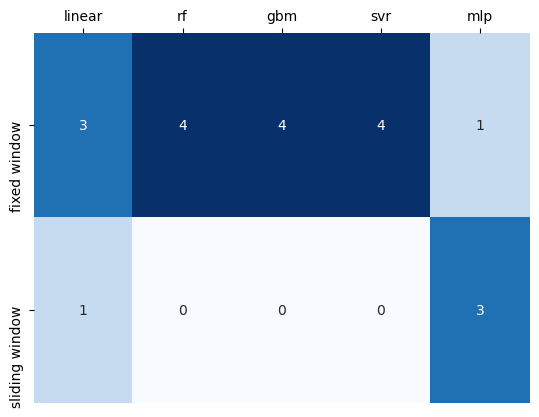
\includegraphics[width=\columnwidth]{figures/first_study/comp_window_mae.png}
\caption{Pairwise systematicity matrix concerning window type for MAE.}
\end{figure}

\begin{figure}[htb!]
    \centering
    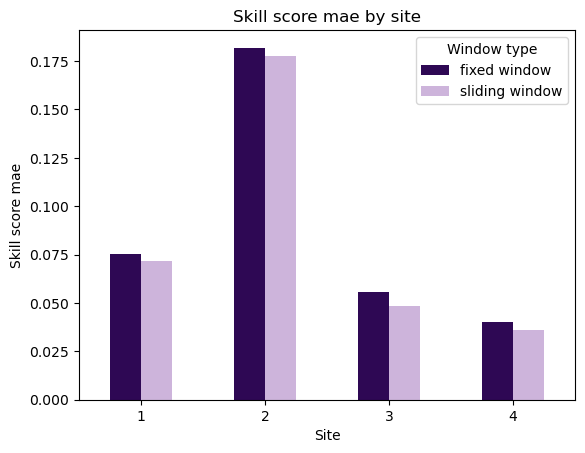
\includegraphics[width=\columnwidth]{figures/first_study/comp_window_mae_svr.png}
\caption{Comparison of the MAE skill scores for a SVR model.}
\end{figure}

Interestingly, the fixed window performs best that the sliding window for all the study cases. 

\paragraph{Influence of the NWP forecasting model}
All the previous optimisations were done on the GFS forecast, as it was explained in \autoref{sec:methodo}.

Reuniwatt uses the data from several different numerical weather prediction (NWP) models, including ECMWF, AROME and ARPEGE.
It is interesting to see how our models perform on this different data source.
\begin{figure}[htb!]
    \centering
    \includesvg[width=\columnwidth]{figures/first_study/comp_for_models_ss_mae.svg}
    \caption{Comparison of the MAE skill scores of the SVR model of four different NWP forecast models.}
    \label{fig:models_ss}   
\end{figure}

\begin{figure}[htb!]
    \centering
    \includesvg[width=\columnwidth]{figures/first_study/comp_for_models_mae.svg}
\caption{Comparison of the post-processing of four different NWP forecast models on MAE.}
\label{fig:models_plot}
\end{figure}

\autoref{fig:models_ss} clearly shows that the NWP models differently benefit from the post-processing.
There seems to be higher skill scores for less elaborate models such as AROME in comparison to more advanced models such as ECMWF. The higher is the raw forecast metrics, the better is the post-processing.

This is confirmed by \autoref{fig_models_plot} where it can be clearly seen that post-processed metrics fall in a much thiner range than the initial one. It is worthwhile to point out that the ECMWF forecast still remains the best forecast after post-processing.\\

Now that each forecast model has been post-processed, it would be interesting to hybride them so as to compare the performances against the current LT CONT model used by Reuniwatt.

Before doing it, we need to find another linear model to compare against the machine-learning models, since the Kalman filter did not prove its effectiveness.
\subsection{Benchmarking the linear regression models}

\paragraph{MAE}
\begin{figure}[htb!]
    \centering
    \includesvg[width=\columnwidth]{figures/linear_study/mae_matrix.svg}
\caption{Significance matrix for MAE. Models at the top of the matrix are the most succesful ones, on the criterium of the sum of the values of each line. The value $V_{(i,j)}$ of the $(i,j)$ cell indicates how often the model of line i performs better than the one of column j, across the 
4 sites. For example, the MAE of the Lars model post-processed data is 1 times lower than the MAE of the Lasso model, and for 1 site (4 - 1 = 3), it is higher.}
\end{figure}

\begin{figure}[htb!]
    \centering
    \includesvg[width=\columnwidth]{figures/linear_study/mae_ss.svg}
\caption{MAE skill score plots of the best linear models.}
\end{figure}


\paragraph{RMSE}
\begin{figure}[htb!]
    \centering
    \includesvg[width=\columnwidth]{figures/linear_study/rmse_matrix.svg}
\caption{Significance matrix for RMSE. Models at the top of the matrix are the most succesful ones, on the criterium of the sum of the values of each line. The value $V_{(i,j)}$ of the $(i,j)$ cell indicates how often the model of line i performs better than the one of column j, across the 
4 sites. For example, the RMSE of the Lars model post-processed data is 1 times lower than the RMSE of the Lasso model, and for 1 site (4 - 1 = 3), it is higher.}
\end{figure}

\begin{figure}[htb!]
    \centering
    \includesvg[width=\columnwidth]{figures/linear_study/rmse_ss.svg}
\caption{RMSE skill score plots of the best linear models.}
\end{figure}
\subsection{Showcase of the hybrid model}
\subsubsection{Study on the four inital sites}
\begin{figure}[htb!]
    \centering
    \includesvg[width=\columnwidth]{figures/final_study/widen_time_window.svg}
\caption{Comparison of the two versions of LT CONT.}
\end{figure}
\paragraph{MAE}
\begin{figure}[htb!]
    \centering
    \includesvg[width=\columnwidth]{figures/final_study/ss_best_mae.svg}
\caption{MAE skill score plots of the relevant models, the reference being here the best NWP forecast (in practise, this means ECMWF).}
\end{figure}

\begin{figure}[htb!]
    \centering
    \includesvg[width=\columnwidth]{figures/final_study/evolution_plot_mae.svg}
\caption{MAE evolution of the relevant models.}
\end{figure}


\paragraph{RMSE}
\begin{figure}[htb!]
    \centering
    \includesvg[width=\columnwidth]{figures/final_study/ss_best_rmse.svg}
\caption{RMSE skill score plots of the relevant models, the reference being here the best NWP forecast (in practise, this means ECMWF).}
\end{figure}

\begin{figure}[htb!]
    \centering
    \includesvg[width=\columnwidth]{figures/final_study/evolution_plot_rmse.svg}
\caption{RMSE evolution of the relevant models.}
\end{figure}

\subsubsection{Study on the German sites}

\begin{figure}[htb!]
    \centering
    \includesvg[width=\columnwidth]{figures/german_sites.svg}
\caption{The 25 German sites used for validation.}

\end{figure}
\paragraph{MAE}
\begin{figure}[htb!]
    \centering
    \includesvg[width=\columnwidth]{figures/final_study/ss_heatmap_mae.svg}
\caption{MAE skill score heatmap of the validation sites.}
\end{figure}
\paragraph{RMSE}
\begin{figure}[htb!]
    \centering
    \includesvg[width=\columnwidth]{figures/final_study/ss_heatmap_rmse.svg}
\caption{RMSE skill score heatmap of the validation sites.}
\end{figure}


\begin{figure}[htb!]
    \centering
    \includesvg[width=\columnwidth]{figures/final_study/ss_heatmap_rmse_linear_4_sites.svg}
\caption{Global linear model verification on the 4 initial sites.}
\end{figure}
\newpage
\section{Conclusions and perspectives}
\subsection{Results summary}
\begin{itemize}
    \item The Kalman filter has not been proven interesting enough for post-processing day-ahead irradiance forecasts, in opposition to what was said in \cite{suksamosorn_post-processing_2021} paper. The difference may be due to the fact that we used a more precise GFS data in comparison to the WRF data used in the paper. What is more, I dealed with the extreme case of day-ahead data with origin 00:00 UTC, while the paper fixed the origin at 13:00 (local hour).

    A more appropriate use of the Kalman filter would be for filtering faulty data, as explored in \cite{sec:filtering}.
    \item For a MAE minimisation, the SVR model clearly yielded the best results, both for post-processing a single NWP model and for hybridation. This confirms \cite{verbois_statistical_2022}.
    \item For a RMSE minimisation, there is no clear consensus for post-processing a single NWP model, as it was the case in the literature where the random forest (\cite{suksamosorn_post-processing_2021}), GBM and MLP models (\cite{verbois_statistical_2022}) were deemed promising. Still the MLP model as well as the linear least square regression model stand out.

    The hybridation showed some limits of the MLP model, in favor of the linear model.
    \item Using the LT CONT model on post-processed data only yielded marginal enhancements in metrics, whereas using the adequate model (SVR for MAE, Linear regression for RMSE) on the whole dataset provided significant improvements as compared to the LT CONT model.
\end{itemize}
\subsection{Suggestions for future improvements}
\subsection{My learnings from the internship}

\bibliographystyle{abbrvnat}
\bibliography{biblio.bib}

\appendix
\end{document}